\beginsong{Jenseits des Tales}[txt={Börries Freiherr von Münchhausen, vermutlich 1924}, mel={Robert Götz, 1932}, bo={216}, pfii={62}, pfiii={72}]

\markboth{\songtitle}{\songtitle}

\beginverse
\endverse

\centering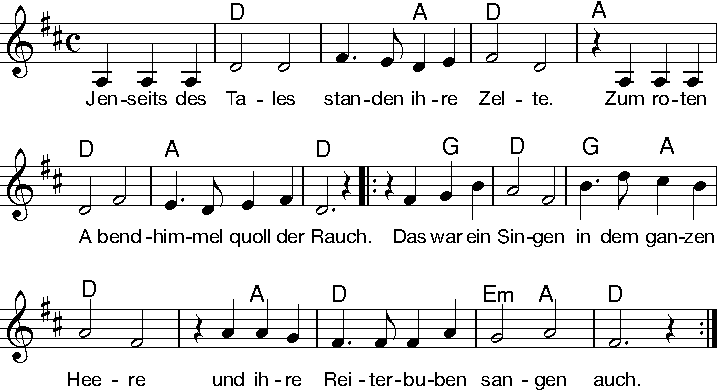
\includegraphics[width=1\textwidth]{Noten/Lied056.pdf}	

\beginverse
Sie putzten \[D]klirrend am \[A]Geschirr der \[D]Pferde, 
\[A]her tänzel\[D]te die \[A]Marketende\[D]rin
\lrep und \[G]unter'm \[D]Singen \[G]sprach der \[A]Knaben \[D]einer: 
''Mäd\[A]chen, du \[D]weißt, wo ging der \[Em]Kö\[A]nig \[D]hin?'' \rrep
\endverse

\beginverse
Diesseits des ^Tales stand der ^junge ^König 
^und griff die ^feuchte ^Erde aus dem ^Grund,
\lrep sie ^kühlte ^nicht die ^Glut der ^heißen ^Stirne,
sie ^machte ^nicht sein krankes ^Herz ^ge^sund. \rrep
\endverse

\beginverse 
Ihn heilten ^nur zwei knaben^frische ^Wangen
^und ein ^Mund, den ^er sich selbst ver^bot.
\lrep Noch ^fester ^schloss der ^König ^seine ^Lippen
und ^sah hi^nüber in das ^A^bend^rot. \rrep
\endverse

\beginverse
Jenseits des ^Tales standen ^ihre ^Zelte,
^zum roten ^Abend^himmel quoll der ^Rauch.
\lrep Und ^war ein ^Lachen ^in dem ^ganzen ^Heere
und ^jener ^Reiterbube ^lach^te ^auch. \rrep
\endverse

\endsong

\beginscripture{}
Das Lied wird scherzhaft auch ''Lied des schwulen Königs'' genannt. Tatsächlich lehnt sich das Lied wohl jedoch an die Ballade vom Reiterjungen an, in der die Geliebte des Königs sich als Junge getarnt ins Heer schmuggelt, um bei ihm sein zu können.
\endscripture

\begin{intersong}

\end{intersong}